\documentclass[conference]{IEEEtran}
\IEEEoverridecommandlockouts

\usepackage[T1]{fontenc}
\usepackage{cite}
\usepackage{amsmath,amssymb}
\usepackage{graphicx}
\usepackage{booktabs}
\usepackage{array}
\usepackage{xcolor}
\usepackage[hidelinks]{hyperref}
\usepackage{enumitem}
\usepackage{tikz}
\usetikzlibrary{shapes.multipart,positioning,arrows.meta,fit,backgrounds,calc}
\usepackage[edges]{forest}

\setlist{leftmargin=*,itemsep=1pt,topsep=2pt}

\definecolor{navy}{HTML}{1B1F3B}
\definecolor{coral}{HTML}{E76F51}
\definecolor{teal}{HTML}{0FA3B1}
\definecolor{blue}{HTML}{3D7DD8}
\definecolor{purple}{HTML}{6C63FF}
\definecolor{tint}{HTML}{F2ECE2}
\definecolor{lgray}{HTML}{F4F4F6}

\tikzset{
  umlclass/.style={rectangle split, rectangle split parts=3, draw=navy, fill=white,
    font=\scriptsize\ttfamily, align=left, inner sep=2pt, rectangle split part fill={tint,white,white},
    text width=#1},
  umlclass/.default=3.1cm,
  inherit/.style={-{Triangle[open,length=2.2mm,width=2.2mm]}, draw=navy},
  assoc/.style={-{Stealth[length=1.8mm]}, draw=navy},
  depend/.style={-{Stealth[length=1.8mm]}, draw=navy, dashed},
  compose/.style={{Diamond[length=2.4mm,width=1.8mm]}-, draw=navy},
  node/.style={draw=#1, fill=#1!8, rounded corners=2pt, font=\scriptsize, align=center,
    inner sep=3pt},
  zone/.style={draw=#1, dashed, rounded corners=4pt, inner sep=5pt},
  flow/.style={-{Stealth[length=1.8mm]}, draw=navy!80},
  lbl/.style={font=\tiny\itshape, fill=white, inner sep=1pt}
}

\begin{document}

\title{TitrateRL: IMRaD Outline, Deployment, Repository Structure, Class Diagram and MVP of a
Simulation-Based Reinforcement Learning Framework for Basal Insulin Titration}

\author{
\IEEEauthorblockN{Boburmirzo Uchqunov}
\IEEEauthorblockA{ID 240447\\ Software engineering,\\ CI, dashboard}
\and
\IEEEauthorblockN{Nodirjon Khabibullaev}
\IEEEauthorblockA{ID 230019\\ Literature, evaluation,\\ statistics}
\and
\IEEEauthorblockN{Ibrohim Abralov}
\IEEEauthorblockA{ID 230129\\ Simulator, cohort,\\ validation}
\and
\IEEEauthorblockN{Abdurashid Abdusattarov}
\IEEEauthorblockA{ID 221229\\ RL agents, rewards,\\ safety shield}
\and
\IEEEauthorblockA{\textit{School of Engineering, BSc in Computer Science, Central Asian University}\\
Team TitrateRL \quad Supervisor: Dr.\ Eugene Castro \quad November 2026}
}

\maketitle

\begin{abstract}
TitrateRL is an open, simulation-based framework in which reinforcement learning (RL) agents
learn to titrate a once-daily basal insulin dose for virtual adults with Type~2 diabetes (T2D)
and are compared with clinical titration algorithms. This report gives the one-page IMRaD
outline of the study, the deployment map, the repository file structure and the class diagram of
the implemented software, and the minimum viable product (MVP) defined with the MoSCoW method,
together with the metrics used to accept the product and to answer the research questions. The
software for every MVP feature is implemented and tested (84 automated tests); the simulator
passes four of the five verification checks, cohort calibration is still open, and the agent
experiments have not been run yet. All work is \emph{in silico} and not intended for clinical
use. Code: \url{https://github.com/Nodirjn/TitrateRL}.
\end{abstract}

\begin{IEEEkeywords}
reinforcement learning, Type 2 diabetes, basal insulin titration, Gymnasium, MVP, MoSCoW
\end{IEEEkeywords}

% =====================================================================================
\section{IMRaD Outline}
\label{sec:imrad}

\subsection{Introduction}
\begin{itemize}
\item \textbf{Context.} 589 million adults live with diabetes, over 90\% with T2D. Basal
insulin (e.g., glargine) is started at 10~U/day and titrated by fasting glucose; at +2~U every
3~days reaching 50~U takes 60~days, and 81\% of patients remain above their HbA1c target after
six months.
\item \textbf{Gap.} Clinical algorithms use one rule for everyone; 24 of 29 RL glucose-control
studies address Type~1 diabetes; no open, RL-ready environment for daily T2D basal titration
exists.
\item \textbf{Aim.} Build an open benchmark and test whether a learned, shielded policy titrates
better than clinical rules. \textbf{RQ1}: effect of the reward (R1 time in range, R2 risk index,
R3 TIR with hypoglycemia penalties). \textbf{RQ2}: $\geq$5~pp more time in range than
AT.LANTUS, Treat-to-Target and INSIGHT with non-inferior hypoglycemia. \textbf{RQ3}: dependence
of the benefit on hidden insulin sensitivity.
\end{itemize}

\subsection{Methods}
\begin{itemize}
\item \textbf{Simulator.} Dalla Man T2D meal model (15 ODE states, RK4, 1-min step, Numba) with
endogenous secretion, two-compartment glargine absorption, meals, CGM and fingerstick noise.
\item \textbf{Cohort.} 150 virtual adults (fasting glucose, weight, insulin-sensitivity and
$\beta$-cell factors), split 90/30/30 by insulin-sensitivity tertile; calibrated against the
Treat-to-Target trial.
\item \textbf{Decision problem.} Partially observable MDP, one step per day, 168-day episodes;
observation = 3-day stack of 11 features; action $\in\{-4,-2,0,+2,+4\}$~U; weekly rate limit
8~U, dose $\leq 1$~U/kg.
\item \textbf{Agents and baselines.} PPO (primary) and DQN (Stable-Baselines3), $10^6$ days per
run, 5 seeds; rule-based safety shield; baselines B0 (fixed), B1--B3 (clinical), B4 (tuned).
\item \textbf{Evaluation.} 30 unseen patients $\times$ 10 scenarios with common random numbers;
noise-free endpoints; one-sided Wilcoxon with Holm correction, Hodges--Lehmann estimate,
bootstrap CIs, Spearman correlation.
\end{itemize}

\subsection{Results (status and expected outputs)}
\begin{itemize}
\item \textbf{Achieved.} All MVP software implemented; 84 tests pass; one 168-day episode runs
in $\approx$0.15~s; PPO trains at $\approx$690 steps/s ($\approx$25~min per $10^6$ steps).
\item \textbf{Verification.} V1 (integrator, equilibrium, dose--response, identical right-hand
side to \texttt{simglucose}) and V2 (flat glargine profile) pass; V4 calibration fails on
fasting glucose (99.6 vs.\ 117~mg/dL in the trial) while the final dose matches (0.57 vs.\
0.48~U/kg).
\item \textbf{Preliminary software check} (validation patients, one scenario): clinical rules
reach a median maintenance TIR of 60--63\% vs.\ 39\% without titration.
\item \textbf{Expected.} Tables of TIR/TBR per reward (RQ1), H2 decision table vs.\ B1--B3
(RQ2), correlation and dose-behaviour plots by insulin-sensitivity tertile (RQ3).
\end{itemize}

\subsection{Discussion (planned)}
\begin{itemize}
\item Interpret efficacy--safety trade-offs of the rewards and the value of CGM features (PPO vs.\
FPG-only PPO) and of learning vs.\ tuning (vs.\ B4).
\item \textbf{Limitations.} No glucagon (hypoglycemia interpreted comparatively); single-meal
model extrapolated to 24 weeks; perfect adherence; calibration gap; sim-to-real gap.
\item \textbf{Contribution.} Open benchmark \texttt{TitrateRL/T2D-v0}, pre-specified comparison,
analysis of personalization. Not a medical device.
\end{itemize}

% =====================================================================================
\section{Deployment Map}
\label{sec:deploy}

Fig.~\ref{fig:deploy} shows where each part of TitrateRL runs and how artifacts move. TitrateRL
has no server back end and handles no personal data: the only deployed units are the Python
package, the experiment runs and the Streamlit dashboard.

\begin{figure*}[t]
\centering
\resizebox{\textwidth}{!}{%
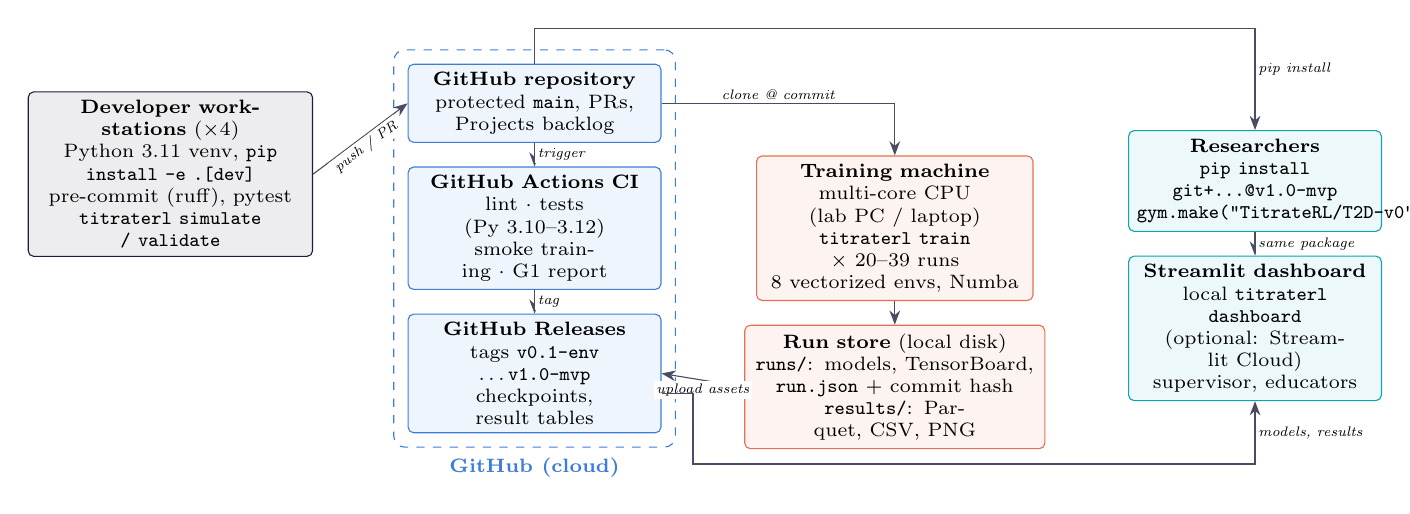
\begin{tikzpicture}[node distance=4mm and 6mm]
% developer workstations
\node[node=navy, text width=3.4cm] (dev) {\textbf{Developer workstations} ($\times$4)\\
Python 3.11 venv, \texttt{pip install -e .[dev]}\\ pre-commit (ruff), pytest\\
\texttt{titraterl simulate / validate}};
% GitHub
\node[node=blue, text width=3.0cm, right=12mm of dev, yshift=9mm] (repo) {\textbf{GitHub repository}\\
protected \texttt{main}, PRs,\\ Projects backlog};
\node[node=blue, text width=3.0cm, below=3mm of repo] (ci) {\textbf{GitHub Actions CI}\\
lint $\cdot$ tests (Py 3.10--3.12)\\ smoke training $\cdot$ G1 report};
\node[node=blue, text width=3.0cm, below=3mm of ci] (rel) {\textbf{GitHub Releases}\\
tags \texttt{v0.1-env} \dots \texttt{v1.0-mvp}\\ checkpoints, result tables};
\begin{scope}[on background layer]
\node[zone=blue, fit=(repo)(ci)(rel), label={[font=\scriptsize\bfseries,text=blue]below:GitHub (cloud)}] (gh) {};
\end{scope}
% training compute
\node[node=coral, text width=3.3cm, right=12mm of ci] (train) {\textbf{Training machine}\\
multi-core CPU (lab PC / laptop)\\ \texttt{titraterl train} $\times$ 20--39 runs\\
8 vectorized envs, Numba};
\node[node=coral, text width=3.6cm, below=3mm of train] (store) {\textbf{Run store} (local disk)\\
\texttt{runs/}: models, TensorBoard,\\ \texttt{run.json} + commit hash\\
\texttt{results/}: Parquet, CSV, PNG};
% users
\node[node=teal, text width=3.0cm, right=12mm of train, yshift=6mm] (pip) {\textbf{Researchers}\\
\texttt{pip install git+\dots@v1.0-mvp}\\ \texttt{gym.make("TitrateRL/T2D-v0")}};
\node[node=teal, text width=3.0cm, below=3mm of pip] (dash) {\textbf{Streamlit dashboard}\\
local \texttt{titraterl dashboard}\\ (optional: Streamlit Cloud)\\ supervisor, educators};
% arrows
\draw[flow] (dev.east) -- node[lbl, below, sloped]{push / PR} (repo.west);
\draw[flow] (repo) -- node[lbl, right]{trigger} (ci);
\draw[flow] (ci) -- node[lbl, right]{tag} (rel);
\draw[flow] (repo.east) -| node[lbl, pos=0.25, above]{clone @ commit} (train.north);
\draw[flow] (train) -- (store);
\draw[flow] (store.west) -- node[lbl, below]{upload assets} (rel.east);
\draw[flow] (rel.east) ++(0,-0.25) -| ++(0.4,-0.9) -| node[lbl, pos=0.75, right]{models, results} (dash.south);
\draw[flow] (repo.north) |- ++(5,0.45) -| node[lbl, pos=0.7, right]{pip install} (pip.north);
\draw[flow] (pip) -- node[lbl, right]{same package} (dash);
\end{tikzpicture}}
\caption{Deployment map. Code flows from the four workstations through pull requests and CI to
tagged releases; experiments run on a multi-core CPU machine from a pinned commit; trained models
and result tables are published as release assets (never committed to git) and consumed by the
dashboard and by researchers who install the package.}
\label{fig:deploy}
\end{figure*}

\begin{itemize}
\item \textbf{Repository.} \url{https://github.com/Nodirjn/TitrateRL} (MIT license).
\item \textbf{Environments.} \emph{Development}: each member's laptop. \emph{CI}: GitHub-hosted
Ubuntu runners, CPU-only PyTorch. \emph{Experiments}: one multi-core CPU machine (no GPU needed;
the networks are $2\times64$ MLPs). \emph{Presentation}: local Streamlit server.
\item \textbf{Reproducibility contract.} A run is identified by its YAML file, seed and commit
hash, recorded in \texttt{run.json}; dependencies are pinned; data and models travel as release
assets.
\item \textbf{Safety.} The dashboard accepts only virtual-patient identifiers and labels every
output as a simulation result.
\end{itemize}

% =====================================================================================
\section{Repository File Structure}
\label{sec:repo}

The repository (Fig.~\ref{fig:tree}) follows the \texttt{src} layout and mirrors the six
architecture layers: configuration and data, simulation core, environment, decision,
evaluation, and presentation. Experiment outputs (\texttt{data/}, \texttt{runs/},
\texttt{results/}, \texttt{reports/}) are generated and git-ignored.

\begin{figure}[t]
\centering
\scriptsize
\begin{forest}
  for tree={font=\ttfamily\scriptsize, grow'=0, folder, s sep=0.6pt, inner sep=0.8pt,
    l sep=6pt, fit=band},
  [titraterl/
    [{.github/ \normalfont\textit{--- CI workflow, PR and issue templates}}]
    [configs/
      [cohort.yaml]
      [{train/ \normalfont\textit{--- ppo\_r1/r2/r3, ppo\_rstar\_shield, dqn, fpg, smoke}}]
      [{eval/ \normalfont\textit{--- test.yaml, baselines\_quick.yaml}}]]
    [src/titraterl/
      [{simulation/ \normalfont\textit{--- parameters, model (ODE, RK4), scenario, sensors, patient}}]
      [{cohort/ \normalfont\textit{--- generator, split, Parquet I/O}}]
      [{envs/ \normalfont\textit{--- titration\_env, observation, rewards, wrappers}}]
      [{policies/ \normalfont\textit{--- base, rules (B0--B4), sb3}}]
      [{training/ \normalfont\textit{--- train, callbacks}}]
      [{metrics/ \normalfont\textit{--- glycemic, episode}}]
      [{evaluation/ \normalfont\textit{--- runner, statistics, logging, pipeline}}]
      [validation/ \normalfont\textit{--- checks V1--V5}]
      [{config.py, cli.py}]]
    [dashboard/app.py]
    [tests/
      [{unit/ \normalfont\textit{--- model, cross-impl., env, shield, rules, ...}}]
      [{integration/ \normalfont\textit{--- pipeline, CLI, training, dashboard}}]]
    [{docs/ \normalfont\textit{--- architecture, model, environment, evaluation, ...}}]
    [{examples/ \normalfont\textit{--- quickstart.py, quickstart.ipynb}}]
    [{README.md, MODEL\_CARD.md, pyproject.toml, Makefile, LICENSE}]
  ]
\end{forest}
\caption{Repository file structure (86 tracked files, $\approx$3\,800 lines of package code and
$\approx$800 lines of tests).}
\label{fig:tree}
\end{figure}

\textbf{Conventions.} GitHub Flow with a protected \texttt{main}; Conventional Commits; one
reviewer per pull request; CI runs ruff and pytest on Python 3.10--3.12; every experiment is a
YAML file; milestones are tags \texttt{v0.1-env}, \texttt{v0.2-agents}, \texttt{v0.3-eval},
\texttt{v1.0-mvp}.

% =====================================================================================
\section{Class Diagram}
\label{sec:classes}

Fig.~\ref{fig:classes} shows the main classes. \texttt{T2DTitrationEnv} composes a
\texttt{VirtualPatient}, which owns the parameter vector, the ODE state and three random streams
(meals, CGM, fingerstick) for common random numbers. Rule-based baselines and RL agents share one
abstract \texttt{Policy} interface, so the evaluator, the statistics module and the dashboard
treat them identically. \texttt{SafetyShield} is a Gymnasium wrapper applied only to RL agents;
the rate limit and dose bounds live in the environment and apply to every policy.

\begin{figure*}[t]
\centering
\resizebox{\textwidth}{!}{%
\begin{tikzpicture}[node distance=5mm and 7mm]
% --- simulation layer
\node[umlclass=3.2cm] (pp) {\textbf{PatientParameters}
\nodepart{second} patient\_id: str\\ body\_weight\_kg: float\\ fpg\_preinsulin: float\\
rho\_si, rho\_beta: float
\nodepart{third} vector(): ndarray\\ initial\_state(): ndarray};
\node[umlclass=3.2cm, below=6mm of pp] (vp) {\textbf{VirtualPatient}
\nodepart{second} p, state: ndarray\\ cgm: CGMSensor\\ meal\_rng, smbg\_rng
\nodepart{third} step\_day(dose\_u): DayResult};
\node[umlclass=3.0cm, below=6mm of vp] (dr) {\textbf{DayResult}
\nodepart{second} glucose\_true[1440]\\ glucose\_cgm[288]\\ fasting\_smbg: float\\ meals: DayMeals
\nodepart{third} glucose\_true\_5min()};
\node[umlclass=2.6cm, left=7mm of vp] (cgm) {\textbf{CGMSensor}
\nodepart{second} params: CGMNoiseParams
\nodepart{third} measure\_day(g): ndarray};
\node[umlclass=2.6cm, above=6mm of cgm] (cp) {\textbf{CohortPatient}
\nodepart{second} params\\ split: str\\ si\_tertile: int
\nodepart{third} patient\_id()};
\node[umlclass=2.6cm, above=6mm of cp] (co) {\textbf{Cohort}
\nodepart{second} patients: list
\nodepart{third} split(name)\\ save(path), load(path)};
% --- environment layer
\node[umlclass=3.4cm, right=10mm of pp, yshift=-4mm] (env) {\textbf{T2DTitrationEnv}\\ \textit{gymnasium.Env}
\nodepart{second} observation\_space: Box(33)\\ action\_space: Discrete(5)\\
dose\_u: float\\ history: list[DayRecord]
\nodepart{third} reset(seed, options)\\ step(action)\\ step\_units(delta\_u)\\
hypo\_level1\_recent(): bool};
\node[umlclass=2.8cm, below=6mm of env] (obs) {\textbf{ObservationStack}
\nodepart{second} mode: full | fpg\_only
\nodepart{third} reset(f), push(f)};
\node[umlclass=2.8cm, below=6mm of obs] (sh) {\textbf{SafetyShield}\\ \textit{gymnasium.Wrapper}
\nodepart{second} config: ShieldConfig\\ interventions: int
\nodepart{third} step(action)};
% --- decision layer
\node[umlclass=3.0cm, right=10mm of env, yshift=6mm] (pol) {\textit{\textbf{Policy}} \{abstract\}
\nodepart{second} policy\_id: str\\ action\_mode, obs\_mode\\ shield: bool
\nodepart{third} initial\_dose(bw): float\\ reset(info)\\ act(obs, info)};
\node[umlclass=2.1cm, below left=9mm and -14mm of pol] (b0) {\textbf{FixedDose}\nodepart{second} B0\nodepart{third} act()};
\node[umlclass=2.3cm, right=2mm of b0] (ir) {\textbf{\_IntervalRule}\nodepart{second} interval\_days\\ target\nodepart{third} act()};
\node[umlclass=2.0cm, right=2mm of ir] (sb3) {\textbf{SB3Policy}\nodepart{second} model: PPO|DQN\nodepart{third} load(path)};
\node[umlclass=2.2cm, below=7mm of b0, xshift=6mm] (t2t) {\textbf{TreatToTarget}\nodepart{second} B2\nodepart{third} act()};
\node[font=\scriptsize\ttfamily, draw=navy, fill=white, align=left, below=7mm of ir, xshift=10mm, text width=2.6cm] (rules)
  {\textbf{ATLantus} (B1)\\ \textbf{Insight} (B3)\\ \textbf{ThresholdRule} (B4)};
% --- evaluation layer
\node[umlclass=3.4cm, below=22mm of t2t, xshift=-12mm] (ev) {\textbf{evaluation.runner}\\ \guillemotleft module\guillemotright
\nodepart{second} \nodepart{third} run\_episode(policy, patient, seed)\\ evaluate(policies, patients, n)\\ per\_patient(df)};
\node[umlclass=3.4cm, right=5mm of ev] (stat) {\textbf{evaluation.statistics}\\ \guillemotleft module\guillemotright
\nodepart{second} \nodepart{third} evaluate\_h1/h2/h3()\\ hodges\_lehmann(), holm()\\ bootstrap\_ci()};
\node[umlclass=3.0cm, right=5mm of stat] (cb) {\textbf{SelectionCallback}\\ \textit{sb3 BaseCallback}
\nodepart{second} best: SelectionScore
\nodepart{third} \_on\_step(): bool};

% --- relations
\draw[compose] (co.south) -- node[lbl,right]{1..150} (cp.north);
\draw[assoc] (cp.east) -- (pp.west);
\draw[assoc] (vp.north) -- (pp.south);
\draw[compose] (vp.west) -- (cgm.east);
\draw[depend] (vp.south) -- node[lbl,right]{creates} (dr.north);
\draw[compose] (env.west) -- node[lbl,above]{1} ($(vp.east)+(0,0.2)$);
\draw[assoc] (env.north) |- node[lbl,pos=0.75,above]{samples from} ($(co.east)+(0,0.25)$);
\draw[compose] (env.south) -- (obs.north);
\draw[assoc] (sh.east) -| node[lbl,pos=0.2,below]{wraps} ($(env.south east)+(-0.2,0)$);
\draw[inherit] (b0.north) -- ++(0,0.3) -| ($(pol.south)+(-0.5,0)$);
\draw[inherit] (ir.north) -- ++(0,0.3) -| (pol.south);
\draw[inherit] (sb3.north) -- ++(0,0.3) -| ($(pol.south)+(0.5,0)$);
\draw[inherit] (t2t.north) -- (t2t.north |- b0.south);
\draw[inherit] (rules.north) -- (rules.north |- ir.south);
\draw[depend] (ev.north) -- ++(0,0.35) -| node[lbl,pos=0.75,right]{uses Policy} ($(sb3.east)+(0.45,0)$) |- (pol.east);
\draw[depend] (ev.west) -| node[lbl,pos=0.3,above]{runs episodes} (sh.south);
\draw[depend] (cb.north) |- node[lbl,pos=0.7,above]{evaluates} ($(sb3.south)+(0.6,-0.2)$) -- ($(sb3.south)+(0.6,0)$);
\draw[depend] (stat.west) -- node[lbl,above]{reads} (ev.east);
\end{tikzpicture}}
\caption{Class diagram of the implemented TitrateRL package (simplified UML). Open triangles:
inheritance; filled diamonds: composition; solid arrows: association; dashed arrows:
dependency. B1, B3 and B4 inherit from \texttt{\_IntervalRule}; B2 from \texttt{Policy}.}
\label{fig:classes}
\end{figure*}

% =====================================================================================
\section{MVP Definition (MoSCoW) and Metrics}
\label{sec:mvp}

The MVP is the minimal set of working features that demonstrates the complete pipeline: virtual
patients $\rightarrow$ training and shielded titration $\rightarrow$ statistical comparison
$\rightarrow$ interactive visualization (Table~\ref{tab:moscow}). \emph{Must} items form the
protected Core tier; \emph{Should} items are dropped in reverse order if milestone M2 is more than
one week late; \emph{Could} items start only if M3 is on time.

\begin{table*}[t]
\centering
\caption{MVP Prioritization with the MoSCoW Method}
\label{tab:moscow}
\scriptsize
\begin{tabular}{@{}p{1.3cm}p{6.2cm}p{6.9cm}p{2.3cm}@{}}
\toprule
\textbf{Priority} & \textbf{Feature} & \textbf{Acceptance criterion} & \textbf{Status} \\
\midrule
\textbf{Must} & F1 T2D simulator and calibrated 150-patient cohort & generated reproducibly from one seed; checks V1--V4 pass & implemented; V4 open \\
\textbf{Must} & F2 Gymnasium environment \texttt{TitrateRL/T2D-v0} & passes \texttt{check\_env}; 168-day episode $<$2~s; rate-limit and shield tests pass & done (0.15~s) \\
\textbf{Must} & F3 Trained agents: PPO with R1--R3 (shield off) and shielded PPO with R$^\star$, 5 seeds each & checkpoints and learning curves stored; selection on validation patients & pipeline done; runs Wk 7--10 \\
\textbf{Must} & F4 Rule-based policies B0--B3 behind the \texttt{Policy} interface & unit tests reproduce the published titration steps & done \\
\textbf{Must} & F5 Evaluation pipeline & one command regenerates metric tables, statistical tests and figures & done \\
\textbf{Must} & F6 Interactive dashboard & select a test patient and $\leq$3 policies; traces, doses, metrics, disclaimer; 24-week re-run $<$5~s; CSV export & done \\
\textbf{Must} & F7 Installable package & \texttt{pip install}; environment registered; documented API and example notebook & done \\
\textbf{Must} & RQ1--RQ3 analyses & H1--H3 decision rules applied to test-cohort data & Wk 10--13 \\
\midrule
\textbf{Should} & DQN agent; FPG-only PPO; $\lambda$ grid for R3; simulator-tuned rule B4; robustness scenario set & completed and reported as exploratory & code ready \\
\textbf{Could} & Oracle per-patient fine-tuning; 2013 hypoglycemia model extensions; LSTM policy; SAC & started only if M3 is on time & --- \\
\textbf{Won't} (this semester) & Real patient data or clinical deployment; Type~1 diabetes, pumps and bolus insulin; exercise, illness, missed injections; offline RL from EHRs; mobile app & out of scope; stated in README and model card & --- \\
\bottomrule
\end{tabular}
\end{table*}

\subsection{Metrics}

Two kinds of metrics are used: \emph{product metrics} accept the software, and \emph{research
metrics} answer the research questions (Table~\ref{tab:metrics}). Research endpoints are computed
from noise-free plasma glucose over the 30 test patients $\times$ 10 scenarios; every patient
contributes one paired value per comparison.

\begin{table}[t]
\centering
\caption{Metrics Used for the MVP}
\label{tab:metrics}
\scriptsize
\setlength{\tabcolsep}{3pt}
\begin{tabular}{@{}p{2.2cm}p{3.6cm}p{2.2cm}@{}}
\toprule
\textbf{Metric} & \textbf{Definition} & \textbf{Target / role} \\
\midrule
\multicolumn{3}{@{}l}{\textit{Product (acceptance)}} \\
Test suite & unit + integration tests in CI & 100\% pass \\
Episode runtime & one 168-day episode & $<$2~s \\
Dashboard re-run & 24-week simulation & $<$5~s \\
Simulator checks & V1--V4 (gate G1) & all pass by Wk~5 \\
Reproducibility & same seed $\Rightarrow$ same trajectory & exact \\
\midrule
\multicolumn{3}{@{}l}{\textit{Research (glycemic)}} \\
TIR & \% time 70--180~mg/dL, weeks 21--24 & $>$70\%; primary efficacy \\
TBR$_{<70}$, TBR$_{<54}$ & \% time below 70 / 54~mg/dL & $<$4\%, $<$1\%; primary safety \\
TAR$_{>180}$, TAR$_{>250}$ & \% time above 180 / 250 & $<$25\%, $<$5\% \\
Mean, CV, GMI & mean, SD/mean, $3.31+0.02392\,\bar G$ & CV $\leq$36\% \\
LBGI, HBGI & Kovatchev risk indices & risk \\
Time-to-target & 3 consecutive fasting values 80--130 & titration speed \\
Nocturnal TBR & 00:00--06:00 & safety \\
Overbasalization & bedtime$-$morning $\geq$50; dose $>$0.5~U/kg & appropriateness \\
Dose burden & final U/kg; changes per week & burden \\
Shield rate & \% days with intervention & safety \\
\midrule
\multicolumn{3}{@{}l}{\textit{Statistical decision rules}} \\
H2 superiority & Holm-adj.\ one-sided Wilcoxon & $p<0.05$ \\
H2 effect size & Hodges--Lehmann TIR gain & $\geq$5~pp \\
H2 non-inferiority & upper 95\% CI of TBR$_{<70}$ diff. & $<$1~pp \\
H3 & Spearman($\rho_{SI}$, $\Delta$TIR) & negative, $p<0.05$ \\
\bottomrule
\end{tabular}
\end{table}

\subsection{Current status against the MVP}
All seven features are implemented, with 84 automated tests (including a cross-implementation
test against \texttt{simglucose} and a smoke PPO training run). Remaining Must work is the
cohort calibration (check V4: week-24 fasting glucose 99.6~mg/dL vs.\ 110--125~mg/dL; 56\% vs.\
25--50\% of patients at target; final dose 0.57~U/kg within range), the 20 Core training runs
($\approx$15 CPU-hours) and the RQ1--RQ3 analyses, following milestones M1 (\texttt{v0.1-env}) to
M4 (\texttt{v1.0-mvp}, Week~14).

\section*{Disclaimer}
TitrateRL is in silico research software. It is not a medical device, and nothing in this report
is medical advice.

\end{document}
